

%% AAPT Physics Olympiad F=ma Questions
%%----------------------------------------


%% this section contains 49 problems


%% PhysicsOlympiad 2015
%%----------------------------------------
\element{aapt}{ %% Olympiad-A5
\begin{question}{Olympiad-2015-Q06}
    Three trolley carts are free to move on a one dimensional frictionless horizontal track.
    Cart $A$ has a mass of \SI{1.9}{\kilo\gram} and an initial speed of \SI{1.7}{\meter\per\second} to the right;
    Cart $B$ has a mass of \SI{1.1}{\kilo\gram} and an initial speed of \SI{2.5}{\meter\per\second} to the left;
    Cart $C$ has a mass of \SI{1.3}{\kilo\gram} and is originally at rest.
    Collisions between carts $A$ and $B$ are perfectly elastic;
        collisions between carts $B$ and $C$ are perfectly inelastic.
    \begin{center}
    \begin{tikzpicture}
        %% Ground
        \draw[ultra thick] (-4,0) -- (4,0);
        %% Cars
        \node[draw,minimum width=1cm,minimum height=1.5em,anchor=south] (A) at (-3,0.2) {\SI{1.9}{\kilo\gram}};
        \node[draw,minimum width=1cm,minimum height=1.5em,anchor=south] (B) at  (0,0.2) {\SI{1.1}{\kilo\gram}};
        \node[draw,minimum width=1cm,minimum height=1.5em,anchor=south] (C) at (+3,0.2) {\SI{1.3}{\kilo\gram}};
        %% Wheels
        \draw (A.south east) ++(-0.15,-0.1) circle (0.1);
        \draw (A.south west) ++(+0.15,-0.1) circle (0.1);
        \draw (B.south east) ++(-0.15,-0.1) circle (0.1);
        \draw (B.south west) ++(+0.15,-0.1) circle (0.1);
        \draw (C.south east) ++(-0.15,-0.1) circle (0.1);
        \draw (C.south west) ++(+0.15,-0.1) circle (0.1);
        %% Labels
        \node[anchor=south] at (A.north) {Cart $A$};
        \node[anchor=south] at (B.north) {Cart $B$};
        \node[anchor=south] at (C.north) {Cart $C$};
        %% Velocity
        \draw[thick,->] (-3.5,-0.5) -- (-2.5,-0.5) node[pos=0.5,anchor=north] {\SI{1.7}{\meter\per\second}};
        \draw[thick,->] (+0.5,-0.5) -- (-0.5,-0.5) node[pos=0.5,anchor=north] {\SI{2.5}{\meter\per\second}};
    \end{tikzpicture}
    \end{center}
    What is the velocity of the center of mass of the system of the three carts after the last collision?
    \begin{multicols}{3}
    \begin{choices}
      \correctchoice{\SI{0.11}{\meter\per\second}}
        \wrongchoice{\SI{0.16}{\meter\per\second}}
        \wrongchoice{\SI{1.4}{\meter\per\second}}
        \wrongchoice{\SI{2.0}{\meter\per\second}}
        \wrongchoice{\SI{3.23}{\meter\per\second}}
    \end{choices}
    \end{multicols}
\end{question}
}

\newcommand{\OlympiadTwentyFifteenQSeven}{
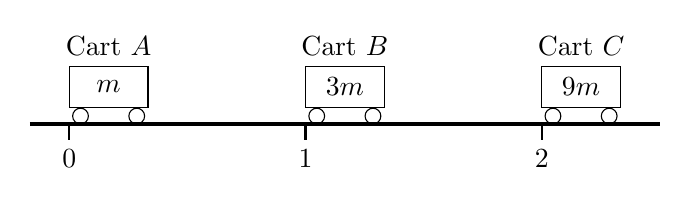
\begin{tikzpicture}
    %% Ground
    \draw[ultra thick] (-4,0) -- (4,0);
    %% Cars
    \node[draw,minimum width=1cm,minimum height=1.5em,anchor=south] (A) at (-3,0.2) {$m$};
    \node[draw,minimum width=1cm,minimum height=1.5em,anchor=south] (B) at  (0,0.2) {$3m$};
    \node[draw,minimum width=1cm,minimum height=1.5em,anchor=south] (C) at (+3,0.2) {$9m$};
    %% Wheels
    \draw (A.south east) ++(-0.15,-0.1) circle (0.1);
    \draw (A.south west) ++(+0.15,-0.1) circle (0.1);
    \draw (B.south east) ++(-0.15,-0.1) circle (0.1);
    \draw (B.south west) ++(+0.15,-0.1) circle (0.1);
    \draw (C.south east) ++(-0.15,-0.1) circle (0.1);
    \draw (C.south west) ++(+0.15,-0.1) circle (0.1);
    %% Labels
    \node[anchor=south] at (A.north) {Cart $A$};
    \node[anchor=south] at (B.north) {Cart $B$};
    \node[anchor=south] at (C.north) {Cart $C$};
    %% Markers
    \draw[thick] (-3.5,0) -- (-3.5,-0.2) node[anchor=north] {\SI{0}{\meter}};
    \draw[thick] (-0.5,0) -- (-0.5,-0.2) node[anchor=north] {\SI{1}{\meter}};
    \draw[thick] (+2.5,0) -- (+2.5,-0.2) node[anchor=north] {\SI{2}{\meter}};
\end{tikzpicture}
}

\element{aapt}{ %% Olympiad-A5
\begin{question}{Olympiad-2015-Q07}
    %% The following information applies to questions 7 and 8
    Carts $A$, $B$, and $C$ are on a long horizontal frictionless track.
    The masses of the carts are $m$, $3m$, and $9m$.
    Originally cart $B$ is at rest at the \SI{1.0}{\meter} mark and cart $C$ is at rest on the \SI{2.0}{\meter} mark.
    Cart $A$ is originally at the zero meter mark moving toward the cart $B$ at a speed of $v_0$.
    \begin{center}
        \OlympiadTwentyFifteenQSeven
    \end{center}
    Assuming that all collisions are completely inelastic,
        what is the final speed of cart $C$?
    \begin{multicols}{3}
    \begin{choices}
      \correctchoice{$\dfrac{1}{13} v_0$}
        \wrongchoice{$\dfrac{1}{10} v_0$}
        \wrongchoice{$\dfrac{1}{9} v_0$}
        \wrongchoice{$\dfrac{1}{3} v_0$}
        \wrongchoice{$\dfrac{2}{5} v_0$}
    \end{choices}
    \end{multicols}
\end{question}
}

\element{aapt}{ %% Olympiad-A5
\begin{question}{Olympiad-2015-Q08}
    %% The following information applies to questions 7 and 8
    Carts $A$, $B$, and $C$ are on a long horizontal frictionless track.
    The masses of the carts are $m$, $3m$, and $9m$.
    Originally cart $B$ is at rest at the \SI{1.0}{\meter} mark and cart $C$ is at rest on the \SI{2.0}{\meter} mark.
    Cart $A$ is originally at the zero meter mark moving toward the cart $B$ at a speed of $v_0$.
    \begin{center}
        \OlympiadTwentyFifteenQSeven
    \end{center}
    Assuming that all collisions are completely elastic,
        what is the final speed of cart $C$?
    \begin{multicols}{3}
    \begin{choices}
        \wrongchoice{$\dfrac{1}{8} v_0$}
      \correctchoice{$\dfrac{1}{4} v_0$}
        \wrongchoice{$\dfrac{1}{2} v_0$}
        \wrongchoice{$ v_0$}
        \wrongchoice{$2 v_0$}
    \end{choices}
    \end{multicols}
\end{question}
}

\element{aapt}{ %% Olympiad-A5
\begin{question}{Olympiad-2015-Q09}
    %The following information applies to questions 9 and 10
    A \SI{0.650}{\kilo\gram} ball moving at \SI{5.00}{\meter\per\second} collides with a \SI{0.750}{\kilo\gram} ball that is originally at rest.
    After the collision,
        the \SI{0.750}{\kilo\gram} ball moves off with a speed of \SI{4.00}{\meter\per\second},
        and the \SI{0.650}{\kilo\gram} ball moves off at a right angle to the final direction of motion of the \SI{0.750}{\kilo\gram} ball.
    %% Start question
    What is the final speed of the \SI{0.650}{\kilo\gram} ball?
    \begin{multicols}{2}
    \begin{choices}
      \correctchoice{\SI{1.92}{\meter\per\second}}
        \wrongchoice{\SI{2.32}{\meter\per\second}}
        \wrongchoice{\SI{3.00}{\meter\per\second}}
        \wrongchoice{\SI{4.64}{\meter\per\second}}
        \wrongchoice{\SI{5.77}{\meter\per\second}}
    \end{choices}
    \end{multicols}
\end{question}
}

\element{aapt}{ %% Olympiad-A5
\begin{question}{Olympiad-2015-Q10}
    %The following information applies to questions 9 and 10
    A \SI{0.650}{\kilo\gram} ball moving at \SI{5.00}{\meter\per\second} collides with a \SI{0.750}{\kilo\gram} ball that is originally at rest.
    After the collision,
        the \SI{0.750}{\kilo\gram} ball moves off with a speed of \SI{4.00}{\meter\per\second},
        and the \SI{0.650}{\kilo\gram} ball moves off at a right angle to the final direction of motion of the \SI{0.750}{\kilo\gram} ball.
    %% Start question
    Let the change in total kinetic energy in this collision be defined by $\Delta K=K_f - K_i$,
        where $K_f$ is the total final kinetic energy,
        and $K_i$ is the total initial kinetic energy.
    Which of the following is true?
    \begin{multicols}{2}
    \begin{choices}
        \wrongchoice{$\Delta K = \dfrac{K_i+K_f}{2}$}
        \wrongchoice{$K_f < \Delta K < K_i$}
        \wrongchoice{$0 < \Delta K < K_f$}
        \wrongchoice{$\Delta K = 0$}
      \correctchoice{$-K_i < \Delta K < 0$}
    \end{choices}
    \end{multicols}
\end{question}
}

\element{aapt}{ %% Olympiad-A5
\begin{question}{Olympiad-2015-Q23}
    A \SI{2.0}{\kilo\gram} object falls from rest a distance of \SI{5.0}{\meter} onto a \SI{6.0}{\kilo\gram} object that is supported by a vertical massless spring with spring constant k = 72 N/m.
    The two objects stick together after the collision,
        which results in the mass/spring system oscillating.
    What is the maximum magnitude of the displacement of the \SI{6.0}{\kilo\gram} object from its original location before it is struck by the falling object?
    \begin{multicols}{3}
    \begin{choices}
        \wrongchoice{\SI{0.27}{\meter}}
      \correctchoice{\SI{1.1}{\meter}}
        \wrongchoice{\SI{2.5}{\meter}}
        \wrongchoice{\SI{2.8}{\meter}}
        \wrongchoice{\SI{3.1}{\meter}}
    \end{choices}
    \end{multicols}
\end{question}
}


%% PhysicsOlympiad 2014
%%----------------------------------------
\element{aapt}{ %% Olympiad-A5
\begin{question}{Olympiad-2014-Q04}
    What are the correct values of the numbers in the following statements?
    Assume there are no external forces,
        and take $N = 1$ to mean that the statement cannot be made for any meaningful number of particles.
    %% NOTE: itemize (sic)
    \begin{itemize}
        \item If a particle at rest explodes into $N_1$ or fewer particles with known masses,
            and the total kinetic energy of the new particles is known,
            the kinetic energy of each of the new particles is completely determined.
        \item If a particle at rest explodes into $N_2$ or fewer particles,
            the velocities of the new particles must lie in a line.
        \item If a particle at rest explodes into $N_3$ or fewer particles,
            the velocities of the new particles must lie in a plane.
    \end{itemize}
    \begin{choices}
        \wrongchoice{$N_1 = 2$, $N_2 = 1$, $N_3 = 1$}
        \wrongchoice{$N_1 = 1$, $N_2 = 2$, $N_3 = 3$}
      \correctchoice{$N_1 = 2$, $N_2 = 2$, $N_3 = 3$}
        \wrongchoice{$N_1 = 3$, $N_2 = 2$, $N_3 = 3$}
        \wrongchoice{$N_1 = 2$, $N_2 = 3$, $N_3 = 4$}
    \end{choices}
\end{question}
}

\element{aapt}{ %% Olympiad-A5
\begin{question}{Olympiad-2014-Q06}
    A cubical box of mass \SI{10}{\kilo\gram} with edge length
        \SI{5}{\meter} is free to move on a frictionless horizontal surface.
    Inside is a small block of mass \SI{2}{\kilo\gram},
        which moves without friction inside the box.
    At time $t=0$,
        the block is moving with velocity \SI{5}{\meter\per\second}
        directly towards one of the faces of the box,
        while the box is initially at rest.
    The coefficient of restitution for any collision between the block and box is \SI{90}{\percent},
        meaning that the relative speed between the box and block immediately after a collision is \SI{90}{\percent} of the relative speed between the box and block immediately before the collision.
    \begin{center}
    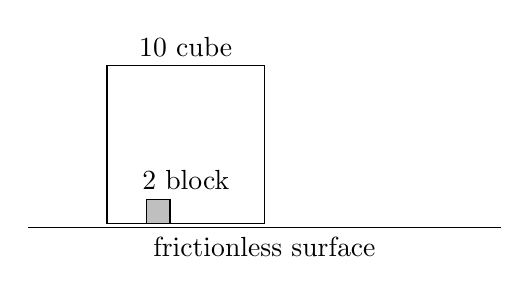
\begin{tikzpicture}
        %% Big box
        \draw (0,0) rectangle (2,2);
        \node[anchor=south] at (1,2) {\SI{10}{\kilo\gram} cube};
        %% small cube
        \draw[fill=white!75!black] (0.5,0) rectangle (0.8,0.3);
        \node[anchor=south] at (1.0,0.3) {\SI{2}{\kilo\gram} block};
        %% Frictionless surface
        \draw (-1,-0.05) -- (5,-0.05) node[pos=0.5,anchor=north] {frictionless surface};
    \end{tikzpicture}
    \end{center}
    After \SI{1}{\minute},
        the block is a displacement $x$ from the original position.
    Which of the following is closest to $x$?
    \begin{multicols}{3}
    \begin{choices}
        \wrongchoice{\SI{0}{\meter}}
      \correctchoice{\SI{50}{\meter}}
        \wrongchoice{\SI{100}{\meter}}
        \wrongchoice{\SI{200}{\meter}}
        \wrongchoice{\SI{300}{\meter}}
    \end{choices}
    \end{multicols}
\end{question}
}

\element{aapt}{ %% Olympiad-A5
\begin{question}{Olympiad-2014-Q16}
    An object of mass $m_1$ initially moving at speed $v_0$
        collides with an object of mass $m_2 = \alpha m_1$,
        where $\alpha <1$, that is initially at rest.
    The collision could be completely elastic, completely inelastic,
        or partially inelastic.
    After the collision the two objects move at speeds $v_1$ and $v_2$.
    Assume that the collision is one dimensional,
        and that object one cannot pass through object two.
    After the collision, the speed ratio $r_1 = \dfrac{v_1}{v_0}$ of object 1 is bounded by:
    \begin{choices}
        \wrongchoice{$\dfrac{1-\alpha}{1+\alpha} \leq r_1 \leq 1$}
      \correctchoice{$\dfrac{1-\alpha}{1+\alpha} \leq r_1 \leq \dfrac{1}{1+\alpha}$}
        \wrongchoice{$\dfrac{\alpha}{1+\alpha} \leq r_1 \leq 1$}
        \wrongchoice{$0 \leq r_1 \leq \dfrac{2\alpha}{1+\alpha}$}
        \wrongchoice{$\dfrac{1}{1+\alpha} \leq r_1 \leq \dfrac{2}{1+\alpha}$}
    \end{choices}
\end{question}
}

\element{aapt}{ %% Olympiad-A5
\begin{question}{Olympiad-2014-Q23}
    A \SI{100}{\kilo\gram} astronaut carries a launcher loaded with a
        \SI{10}{\kilo\gram} bowling ball;
        the launcher and the astronaut's spacesuit have negligible mass.
    The astronaut discovers that firing the launcher results in the ball
        moving away from her at a relative speed of \SI{50}{\meter\per\second}.
    %% Start question
    What is the impulse delivered to the astronaut when firing the launcher?
    \begin{multicols}{2}
    \begin{choices}
      \correctchoice{\SI{455}{\newton\second}}
        \wrongchoice{\SI{500}{\newton\second}}
        \wrongchoice{\SI{550}{\newton\second}}
        \wrongchoice{\SI{5000}{\newton\second}}
        \wrongchoice{\SI{5500}{\newton\second}}
    \end{choices}
    \end{multicols}
\end{question}
}

\element{aapt}{ %% Olympiad-A5
\begin{question}{Olympiad-2014-Q24}
    A \SI{100}{\kilo\gram} astronaut carries a launcher loaded with a
        \SI{10}{\kilo\gram} bowling ball;
        the launcher and the astronaut's spacesuit have negligible mass.
    The astronaut discovers that firing the launcher results in the ball
        moving away from her at a relative speed of \SI{50}{\meter\per\second}.
    %% Start question
    The astronaut is now moving at \SI{10}{\meter\per\second}
        (as measured in a certain frame of reference).
    She wishes to fire the launcher so that her velocity turns through
        as large an angle as possible (in this frame of reference).
    What is this maximum angle?
    (\emph{Hint:} a diagram may be useful.)
    \begin{multicols}{3}
    \begin{choices}
        \wrongchoice{\ang{24.4}}
        \wrongchoice{\ang{26.6}}
      \correctchoice{\ang{27.0}}
        \wrongchoice{\ang{30.0}}
        \wrongchoice{\ang{180.0}}
    \end{choices}
    \end{multicols}
\end{question}
}


%% PhysicsOlympiad 2013
%%----------------------------------------
\element{aapt}{ %% Olympiad-A5
\begin{question}{Olympiad-2013-Q02}
    Jordi stands \SI{20}{\meter} from a wall and Diego stands \SI{10}{\meter} from the same wall.
    Jordi throws a ball at an angle of \ang{30} above the horizontal,
        and it collides elastically with the wall.
    How fast does Jordi need to throw the ball so that Diego will catch it?
    Consider Jordi and Diego to be the same height,
        and both are on the same perpendicular line from the wall.
    \begin{multicols}{3}
    \begin{choices}
        \wrongchoice{\SI{11}{\meter\per\second}}
        \wrongchoice{\SI{15}{\meter\per\second}}
      \correctchoice{\SI{19}{\meter\per\second}}
        \wrongchoice{\SI{30}{\meter\per\second}}
        \wrongchoice{\SI{35}{\meter\per\second}}
    \end{choices}
    \end{multicols}
\end{question}
}

\element{aapt}{ %% Olympiad-A5
\begin{question}{Olympiad-2013-Q07}
    A light car and a heavy truck have the same momentum.
    The truck weighs ten times as much as the car.
    How do their kinetic energies compare?
    \begin{choices}
        \wrongchoice{The truck's kinetic energy is larger by a factor of \num{100}}
        \wrongchoice{They truck's kinetic energy is larger by a factor of \num{10}}
        \wrongchoice{They have the same kinetic energy}
      \correctchoice{The car's kinetic energy is larger by a factor of \num{10}}
        \wrongchoice{The car's kinetic energy is larger by a factor of \num{100}}
    \end{choices}
\end{question}
}

\element{aapt}{ %% Olympiad-A5
\begin{question}{Olympiad-2013-Q08}
    A truck is initially moving at velocity $v$.
    The driver presses the brake in order to slow the truck to a stop.
    The brake applies a constant force $F$ to the truck.
    The truck rolls a distance $x$ before coming to a stop,
        and the time it takes to stop is $t$.
    %% Start question
    Which of the following expressions is equal the initial kinetic energy of the truck
        (i.e. the kinetic energy before the driver starts braking)?
    \begin{multicols}{2}
    \begin{choices}
      \correctchoice{$Fx$}
        \wrongchoice{$Fvt$}
        \wrongchoice{$Fxt$}
        \wrongchoice{$Ft$}
        \wrongchoice{Both $Fx$ and $FvT$ are correct}
    \end{choices}
    \end{multicols}
\end{question}
}

\element{aapt}{ %% Olympiad-A5
\begin{question}{Olympiad-2013-Q09}
    A truck is initially moving at velocity $v$.
    The driver presses the brake in order to slow the truck to a stop.
    The brake applies a constant force $F$ to the truck.
    The truck rolls a distance $x$ before coming to a stop,
        and the time it takes to stop is $t$.
    %% Start question
    Which of the following expressions is equal the initial momentum of the truck
        (i.e. the momentum before the driver starts braking)?
    \begin{multicols}{3}
    \begin{choices}
        \wrongchoice{$Fx$}
        \wrongchoice{$F\dfrac{t}{2}$}
        \wrongchoice{$Fxt$}
        \wrongchoice{$2Ft$}
      \correctchoice{$2F\dfrac{x}{v}$}
    \end{choices}
    \end{multicols}
\end{question}
}

\element{aapt}{ %% Olympiad-A5
\begin{question}{Olympiad-2013-Q14}
    A cart of mass $m$ moving at \SI{12}{\meter\per\second} to the right collides elastically with a cart of mass \SI{4.0}{\kilo\gram} that is originally at rest.
    After the collision,
        the cart of mass $m$ moves to the left with a velocity of \SI{6.0}{\meter\per\second}.
    Assuming an elastic collision in one dimension only,
        what is the velocity of the center of mass ($v_{cm}$) of the two carts before the collision?
    \begin{multicols}{2}
    \begin{choices}
        \wrongchoice{$v_{cm} = \SI{2.0}{\meter\per\second}$}
      \correctchoice{$v_{cm} = \SI{3.0}{\meter\per\second}$}
        \wrongchoice{$v_{cm} = \SI{6.0}{\meter\per\second}$}
        \wrongchoice{$v_{cm} = \SI{9.0}{\meter\per\second}$}
        \wrongchoice{$v_{cm} = \SI{18}{\meter\per\second}$}
    \end{choices}
    \end{multicols}
\end{question}
}

\element{aapt}{ %% Olympiad-A5
\begin{question}{Olympiad-2013-Q18}
    Two point particles, each of mass \SI{1}{\kilo\gram}, begin in the state shown below.
    \begin{center}
    \begin{tikzpicture}[scale=0.9]
        \begin{axis}[
            xlabel={$x$},
            x unit=\si{\meter},
            xtick={-3,-2,-1,0,1,2,3},
            ylabel={$y$},
            y unit=\si{\meter},
            ytick={-3,-2,-1,0,1,2,3},
            grid=major,
            xmin=-3,xmax=3,
            ymin=-3,ymax=3,
            width=0.80\columnwidth,
            height=0.80\columnwidth,
        ]
        \draw[fill] (axis cs:1,1) circle (1.5pt);
        \draw[thick,->] (axis cs:1,1) -- (axis cs:0,1) node[pos=0.5,anchor=south] {\SI{1.0}{\meter\per\second}};
        \draw[fill] (axis cs:1,-1) circle (1.5pt);
        \draw[thick,->] (axis cs:1,-1) -- (axis cs:2,-1) node[pos=0.5,anchor=south] {\SI{1.0}{\meter\per\second}};
        \end{axis}
    \end{tikzpicture}
    \end{center}
    The system evolves through internal forces only.
    Which of the following could be the state after some time has passed?
    %% added to improve printing
    [Axis grid lines in options are identical to those in problem.]
    \begin{multicols}{2}
    \begin{choices}
        \AMCboxDimensions{down=-0.40\columnwidth}
        \wrongchoice{
            \begin{tikzpicture}[font=\small]
                \begin{axis}[
                    clip=false,
                    xlabel={},
                    xtick={-3,-2,-1,0,1,2,3},
                    xticklabels=\empty,
                    ylabel={},
                    ytick={-3,-2,-1,0,1,2,3},
                    yticklabels=\empty,
                    grid=major,
                    xmin=-3,xmax=3,
                    ymin=-3,ymax=3,
                    width=\columnwidth,
                    height=\columnwidth,
                ]
                \draw[fill] (axis cs:-1,0) circle (1.5pt);
                \draw[thick,->] (axis cs:-1,0) -- (axis cs:-1,-1) node[pos=1.0,anchor=north] {\SI{1.0}{\meter\per\second}};
                \draw[fill] (axis cs:1,0) circle (1.5pt);
                \draw[thick,->] (axis cs:1,0) -- (axis cs:1,1) node[pos=1.0,anchor=south] {\SI{1.0}{\meter\per\second}};
                \end{axis}
            \end{tikzpicture}
        }
        \wrongchoice{
            \begin{tikzpicture}[font=\small]
                \begin{axis}[
                    clip=false,
                    xlabel={},
                    xtick={-3,-2,-1,0,1,2,3},
                    xticklabels=\empty,
                    ylabel={},
                    ytick={-3,-2,-1,0,1,2,3},
                    yticklabels=\empty,
                    grid=major,
                    xmin=-3,xmax=3,
                    ymin=-3,ymax=3,
                    width=\columnwidth,
                    height=\columnwidth,
                ]
                \draw[fill] (axis cs:1,1) circle (1.5pt);
                \draw[thick,->] (axis cs:1,1) -- (axis cs:-1,1) node[pos=0.5,anchor=south] {\SI{2.0}{\meter\per\second}};
                \draw[fill] (axis cs:1,-1) circle (1.5pt);
                \end{axis}
            \end{tikzpicture}
        }
        \wrongchoice{
            \begin{tikzpicture}[font=\small]
                \begin{axis}[
                    clip=false,
                    xlabel={},
                    xtick={-3,-2,-1,0,1,2,3},
                    xticklabels=\empty,
                    ylabel={},
                    ytick={-3,-2,-1,0,1,2,3},
                    yticklabels=\empty,
                    grid=major,
                    xmin=-3,xmax=3,
                    ymin=-3,ymax=3,
                    width=\columnwidth,
                    height=\columnwidth,
                ]
                \draw[fill] (axis cs:2,0) circle (1.5pt);
                \draw[thick,->] (axis cs:2,0) -- (axis cs:1.303,0.707) node[pos=1.0,anchor=south] {\SI{1.0}{\meter\per\second}};
                \draw[fill] (axis cs:0,0) circle (1.5pt);
                \draw[thick,->] (axis cs:0,0) -- (axis cs:+0.707,-0.707) node[pos=0.5,anchor=north east] {\SI{1.0}{\meter\per\second}};
                \end{axis}
            \end{tikzpicture}
        }
        \wrongchoice{
            \begin{tikzpicture}[font=\small]
                \begin{axis}[
                    clip=false,
                    xlabel={},
                    xtick={-3,-2,-1,0,1,2,3},
                    xticklabels=\empty,
                    ylabel={},
                    ytick={-3,-2,-1,0,1,2,3},
                    yticklabels=\empty,
                    grid=major,
                    xmin=-3,xmax=3,
                    ymin=-3,ymax=3,
                    width=\columnwidth,
                    height=\columnwidth,
                ]
                \draw[fill] (axis cs:0,2) circle (1.5pt);
                \draw[thick,->] (axis cs:0,2) -- (axis cs:-1,2) node[pos=0.5,anchor=south] {\SI{1.0}{\meter\per\second}};
                \draw[fill] (axis cs:2,-2) circle (1.5pt);
                \draw[thick,->] (axis cs:2,-2) -- (axis cs:3,-2) node[pos=0.5,anchor=south] {\SI{1.0}{\meter\per\second}};
                \end{axis}
            \end{tikzpicture}
        }
        %% ANS is E
        \correctchoice{
            \begin{tikzpicture}[font=\small]
                \begin{axis}[
                    clip=false,
                    xlabel={},
                    xtick={-3,-2,-1,0,1,2,3},
                    xticklabels=\empty,
                    ylabel={},
                    ytick={-3,-2,-1,0,1,2,3},
                    yticklabels=\empty,
                    grid=major,
                    xmin=-3,xmax=3,
                    ymin=-3,ymax=3,
                    width=\columnwidth,
                    height=\columnwidth,
                ]
                \draw[fill] (axis cs:2,1) circle (1.5pt);
                \draw[thick,->] (axis cs:2,1) -- (axis cs:2,2) node[pos=0.5,anchor=east] {\SI{1.0}{\meter\per\second}};
                \draw[fill] (axis cs:0,-1) circle (1.5pt);
                \draw[thick,->] (axis cs:0,-1) -- (axis cs:0,-2) node[pos=0.5,anchor=west] {\SI{1.0}{\meter\per\second}};
                \end{axis}
            \end{tikzpicture}
        }
    \end{choices}
    \end{multicols}
\end{question}
}


%% PhysicsOlympiad 2012
%%----------------------------------------
\element{aapt}{ %% Olympiad-A5
\begin{question}{Olympiad-2012-Q04}
    A particle at rest explodes into three particles of equal mass
        in the absence of external forces.
    Two particles emerge at a right angle to each other with equal speed $v$.
    What is the speed of the third particle?
    \begin{multicols}{2}
    \begin{choices}
        \wrongchoice{$v$}
      \correctchoice{$\sqrt{2}v$}
        \wrongchoice{$2v$}
        \wrongchoice{$2\sqrt{2}v$}
        \wrongchoice{The third particle can have a range of different speeds.}
    \end{choices}
    \end{multicols}
\end{question}
}

\element{aapt}{ %% Olympiad-A5
\begin{question}{Olympiad-2012-Q05}
    A \SI{12}{\kilo\gram} block moving east at \SI{4}{\meter\per\second}
        collides head on with a \SI{6}{\kilo\gram} block that is moving
        west at \SI{2}{\meter\per\second}.
    The two blocks move together after the collision.
    What is the loss in kinetic energy in this collision?
    \begin{multicols}{3}
    \begin{choices}
        \wrongchoice{\SI{36}{\joule}}
        \wrongchoice{\SI{48}{\joule}}
        \wrongchoice{\SI{60}{\joule}}
      \correctchoice{\SI{72}{\joule}}
        \wrongchoice{\SI{96}{\joule}}
    \end{choices}
    \end{multicols}
\end{question}
}


%% PhysicsOlympiad 2011
%%----------------------------------------
\element{aapt}{ %% Olympiad-A5
\begin{question}{Olympiad-2011-Q06}
    A child is sliding out of control with velocity $v_c$ across a frozen lake.
    He runs head-on into another child, initially at rest,
        with \num{3} times the mass of the first child,
        who holds on so that the two now slide together.
    What is the velocity of the couple after the collision?
    \begin{multicols}{3}
    \begin{choices}
        \wrongchoice{$2v_c$}
        \wrongchoice{$v_c$}
        \wrongchoice{$\dfrac{v_c}{2}$}
        \wrongchoice{$\dfrac{v_c}{3}$}
      \correctchoice{$\dfrac{v_c}{4}$}
    \end{choices}
    \end{multicols}
\end{question}
}


%% PhysicsOlympiad 2010
%%----------------------------------------
\element{aapt}{ %% Olympiad-A5
\begin{question}{Olympiad-2010-Q14}
    A \SI{5.0}{\kilo\gram} block with a speed of \SI{8.0}{\meter\per\second}
        travels \SI{2.0}{\meter} along a horizontal surface where it makes a head-on,
        perfectly elastic collision with a \SI{15.0}{\kilo\gram} block which is at rest.
    The coefficient of kinetic friction between both blocks and
        the surface is \num{0.35}.
    How far does the \SI{15.0}{\kilo\gram} block travel before coming to rest?
    \begin{multicols}{2}
    \begin{choices}
        \wrongchoice{$\SI{0.76}{\meter}$}
      \correctchoice{$\SI{1.79}{\meter}$}
        \wrongchoice{$\SI{2.29}{\meter}$}
        \wrongchoice{$\SI{3.04}{\meter}$}
        \wrongchoice{$\SI{9.14}{\meter}$}
    \end{choices}
    \end{multicols}
\end{question}
}

\newcommand{\olympiadTwentyTenQFifteen}{
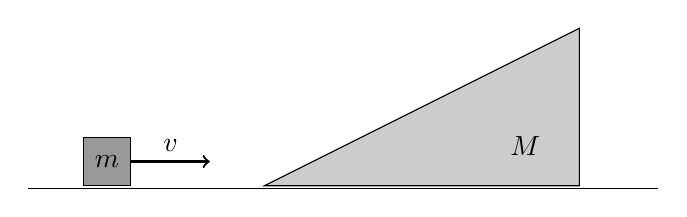
\begin{tikzpicture}
    %% Surface
    \draw (-3,-1pt) -- (5,-1pt);
    %% small block
    \node[draw,fill=white!60!black,rectangle,minimum size=0.6cm,anchor=south] (M) at (-2,0) {$m$};
    \draw[thick,->] (M.east) -- ++(0:1) node[pos=0.5,anchor=south] {$v$};
    %% big block
    \draw[fill=white!80!black] (0,0) -- (4,2) -- (4,0) -- cycle;
    \node[anchor=west] at (3,0.5) {$M$};
\end{tikzpicture}
}

\element{aapt}{ %% Olympiad-A5
\begin{question}{Olympiad-2010-Q15}
    A small block of mass $m$ is moving on a horizontal
        table surface at initial speed $v_0$.
    It then moves smoothly onto a sloped big block of mass $M$.
    The big block can also move on the table surface.
    Assume that everything moves without friction.
    \begin{center}
        \olympiadTwentyTenQFifteen
    \end{center}
    A small block moving with initial speed $v_0$ moves smoothly
        onto a sloped big block of mass $M$.
    After the small block reaches the height $h$ on the slope,
        it slides down.
    Find the height $h$.
    \begin{multicols}{2}
    \begin{choices}
        \wrongchoice{$h=\dfrac{v_0^2}{2g}$}
        \wrongchoice{$h=\dfrac{1}{g}\dfrac{Mv_0^2}{m+M}$}
      \correctchoice{$h=\dfrac{1}{2g}\dfrac{Mv_0^2}{m+M}$}
        \wrongchoice{$h=\dfrac{1}{2g}\dfrac{mv_0^2}{m+M}$}
        \wrongchoice{$h=\dfrac{v_0^2}{g}$}
    \end{choices}
    \end{multicols}
\end{question}
}

\element{aapt}{ %% Olympiad-A5
\begin{question}{Olympiad-2010-Q16}
    A small block of mass $m$ is moving on a horizontal
        table surface at initial speed $v_0$.
    It then moves smoothly onto a sloped big block of mass $M$.
    The big block can also move on the table surface.
    Assume that everything moves without friction.
    \begin{center}
        \olympiadTwentyTenQFifteen
    \end{center}
    A small block moving with initial speed $v_0$ moves smoothly
        onto a sloped big block of mass $M$.
    After the small block reaches the height $h$ on the slope,
        it slides down.
    Following the previous set up,
        find the speed $v$ of the small block after it leaves the slope.
    \begin{multicols}{2}
    \begin{choices}
        \wrongchoice{$v=v_0^2$}
        \wrongchoice{$v=\dfrac{m}{m+M} v_0^2$}
        \wrongchoice{$v=\dfrac{M}{m+M} v_0^2$}
        \wrongchoice{$v=\dfrac{M-m}{m} v_0^2$}
      \correctchoice{$v=\dfrac{M-m}{m+M} v_0^2$}
    \end{choices}
    \end{multicols}
\end{question}
}


%% PhysicsOlympiad 2009
%%----------------------------------------
\newcommand{\olympiadTwentyZeroNineQTwo}{
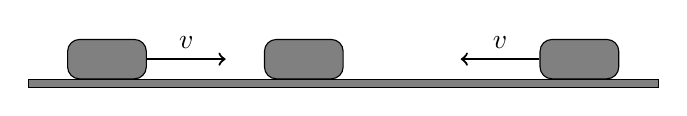
\begin{tikzpicture}
    %% Floor
    \draw[fill=white!50!black] (-4,0) rectangle (4,-0.1);
    %% Blocks
    \node[draw,anchor=south,fill=white!50!black,rounded corners=1ex,minimum width=1cm,minimum height=0.5cm] (A) at (-3,0) {};
    \node[draw,anchor=south,fill=white!50!black,rounded corners=1ex,minimum width=1cm,minimum height=0.5cm] (B) at (-0.5,0) {};
    \node[draw,anchor=south,fill=white!50!black,rounded corners=1ex,minimum width=1cm,minimum height=0.5cm] (C) at (+3,0) {};
    %% Vectors
    \draw[thick,->] (A.east) -- ++(0:1) node[pos=0.5,anchor=south] {$v$};
    \draw[thick,->] (C.west) -- ++(180:1) node[pos=0.5,anchor=south] {$v$};
\end{tikzpicture}
}

\element{aapt}{ %% Olympiad-A5
\begin{question}{Olympiad-2009-Q02}
    Three blocks of identical mass are placed on a frictionless table as shown.
    The center block is at rest,
        whereas the other two blocks are moving directly towards it at identical speeds $v$.
    The center block is initially closer to the left block than the right one.
    All motion takes place along a single horizontal line.
    \begin{center}
        \olympiadTwentyZeroNineQTwo
    \end{center}
    Suppose that all collisions are instantaneous and perfectly elastic.
    After a long time, which of the following is true?
    \begin{choices}
        \wrongchoice{The center block is moving to the left.}
        \wrongchoice{The center block is moving to the right.}
        \wrongchoice{The center block is at rest somewhere to the left of its initial position.}
      \correctchoice{The center block is at rest at its initial position.}
        \wrongchoice{The center block is at rest somewhere to the right of its initial position.}
    \end{choices}
\end{question}
}

\element{aapt}{ %% Olympiad-A5
\begin{question}{Olympiad-2009-Q03}
    Three blocks of identical mass are placed on a frictionless table as shown.
    The center block is at rest,
        whereas the other two blocks are moving directly towards it at identical speeds $v$.
    The center block is initially closer to the left block than the right one.
    All motion takes place along a single horizontal line.
    \begin{center}
        \olympiadTwentyZeroNineQTwo
    \end{center}
    Suppose, instead, that all collisions are instantaneous and perfectly inelastic.
    After a long time, which of the following is true?
    \begin{choices}
        \wrongchoice{The center block is moving to the left.}
        \wrongchoice{The center block is moving to the right.}
        \wrongchoice{The center block is at rest somewhere to the left of its initial position.}
        \wrongchoice{The center block is at rest at its initial position.}
      \correctchoice{The center block is at rest somewhere to the right of its initial position}
    \end{choices}
\end{question}
}

\element{aapt}{ %% Olympiad-A5
\begin{question}{Olympiad-2009-Q14}
    A wooden block (mass $M$) is hung from a peg by a massless rope.
    A speeding bullet (with mass $m$ and initial speed $v_0$)
        collides with the block at time $t=0$ and embeds in it.
    Let $S$ be the system consisting of the block and bullet.
    \begin{center}
    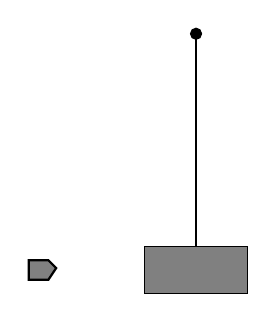
\begin{tikzpicture}
        %% Block
        \node[draw,fill=white!50!black,rectangle,minimum height=0.6cm,minimum width=1.3cm,anchor=center] (M) at (0,0) {};
        \draw (M.north) -- (0,3);
        \draw[fill] (0,3) circle (2pt);
        %% Bullet
        \node[rectangle,minimum size=0.2cm,anchor=center] (B) at (-2,0) {};
        \draw[thick,fill=white!50!black] (B.north east) -- ++(315:0.141) -- (B.south east) -- (B.south west) -- (B.north west) -- (B.north east) -- cycle;
    \end{tikzpicture}
    \end{center}
    Which quantities are conserved between $t=\SI{-10}{\second}$
        and $t=\SI{+10}{\second}$?
    \begin{choices}
        \wrongchoice{The total linear momentum of $S$.}
        \wrongchoice{The horizontal component of the linear momentum of $S$.}
        \wrongchoice{The mechanical energy of $S$.}
        \wrongchoice{The angular momentum of $S$ as measured about a perpendicular axis through the peg.}
      \correctchoice{None of the provided are conserved.}
    \end{choices}
\end{question}
}

\element{aapt}{ %% Olympiad-A5
\begin{question}{Olympiad-2009-Q20}
    Consider a completely inelastic collision between two lumps of space goo.
    Lump 1 has mass $m$ and originally moves directly north with a speed $v_0$.
    Lump 2 has mass $3m$ and originally moves directly east with speed $\dfrac{v_0}{2}$.
    What is the final speed of the masses after the collision?
    Ignore gravity, and assume the two lumps stick together after the collision.
    \begin{multicols}{3}
    \begin{choices}
        \wrongchoice{$\dfrac{7}{16}v_0$}
        \wrongchoice{$\sqrt{\dfrac{5}{8}}v_0$}
      \correctchoice{$\dfrac{\sqrt{13}v_0}{8}$}
        \wrongchoice{$\dfrac{5}{8}v_0$}
        \wrongchoice{$\sqrt{\dfrac{13}{8}}v_0$}
    \end{choices}
    \end{multicols}
\end{question}
}


%% PhysicsOlympiad 2008
%%----------------------------------------
\element{aapt}{ %% Olympiad-A5
\begin{question}{Olympiad-2008-Q07}
    A toboggan sled is traveling at \SI{2.0}{\meter\per\second} across the snow.
    The sled and its riders have a combined mass of \SI{120}{\kilo\gram}.
    Another child ($m_{child}=\SI{40}{\kilo\gram}$) headed
        in the opposite direction jumps on the sled from the front.
    She has a speed of \SI{5.0}{\meter\per\second} immediately before she lands on the sled.
    What is the new speed of the sled?
    Neglect any effects of friction.
    \begin{multicols}{2}
    \begin{choices}
      \correctchoice{\SI{0.25}{\meter\per\second}}
        \wrongchoice{\SI{0.33}{\meter\per\second}}
        \wrongchoice{\SI{2.75}{\meter\per\second}}
        \wrongchoice{\SI{3.04}{\meter\per\second}}
        \wrongchoice{\SI{3.67}{\meter\per\second}}
    \end{choices}
    \end{multicols}
\end{question}
}

\element{aapt}{ %% Olympiad-A5
\begin{questionmult}{Olympiad-2008-Q09}
    A ball of mass $m_1$ travels along the $x$-axis in the positive direction
        with an initial speed of $v_0$.
    It collides with a ball of mass $m_2$ that is originally at rest.
    After the collision, the ball of mass $m_1$ has velocity
        $v_{1x}\hat{x} + v_{1y}\hat{y}$ and the ball of mass $m_2$
        has velocity $v_{2x}\hat{x} + v_{2y}\hat{y}$.
    %Consider the following five statements:
    %\begin{itemize}
    %    \item[I)] $0 = m_1 v_{1x} + m_1 v_{2x}$
    %    \item[II)] $m_1 v_0 = m_1 v_{1y} + m_2 v_{2y}$
    %    \item[III)] $0 = m_1 v_{1y} + m_2 v_{2y}$
    %    \item[IV)] $m_1 v_0 = m_1 v_{1x} + m_1 v_{1y}$
    %    \item[V)] $m_1 v_0 = m_1 v_{1x} + m_2 v_{2x}$
    %\end{itemize}
    Of these five statements, the system must satisfy
    \begin{choices}
        \wrongchoice{$0 = m_1 v_{1x} + m_1 v_{2x}$}
        \wrongchoice{$m_1 v_0 = m_1 v_{1y} + m_2 v_{2y}$}
      \correctchoice{$0 = m_1 v_{1y} + m_2 v_{2y}$}
        \wrongchoice{$m_1 v_0 = m_1 v_{1x} + m_1 v_{1y}$}
      \correctchoice{$m_1 v_0 = m_1 v_{1x} + m_2 v_{2x}$}
        %\wrongchoice{I and II}
        %\correctchoice{III and V}
        %\wrongchoice{II and V}
        %\wrongchoice{III and IV}
        %\wrongchoice{I and III}
    \end{choices}
\end{questionmult}
}

\element{aapt}{ %% Olympiad-A5
\begin{question}{Olympiad-2008-Q22}
    A bullet of mass $m_1$ strikes a pendulum of mass $m_2$ suspended from
        a pivot by a string of length $L$ with a horizontal velocity $v_0$.
    The collision is perfectly inelastic and the bullet sticks to the bob.
    Find the minimum velocity $v_0$ such that the bob (with the bullet inside)
        completes a circular vertical loop.
    \begin{choices}
        \wrongchoice{$2\sqrt{Lg}$}
        \wrongchoice{$\sqrt{5Lg}$}
        \wrongchoice{$\dfrac{m_1+m_2}{m_1} 2\sqrt{Lg}$}
        \wrongchoice{$\dfrac{m_1+m_2}{m_2} \sqrt{Lg}$}
      \correctchoice{$\dfrac{m_1+m_2}{m_1} \sqrt{5Lg}$}
    \end{choices}
\end{question}
}


%% PhysicsOlympiad 2007
%%----------------------------------------
\element{aapt}{ %% Olympiad-A5
\begin{question}{Olympiad-2007-Q09}
    A large wedge rests on a horizontal frictionless surface, as shown.
    \begin{center}
    \begin{tikzpicture}
        %% Ground
        \draw (-1,0) -- (5,0);
        \node[anchor=north,fill,pattern=north east lines,minimum width=6cm, minimum height=0.05cm] at (2,0) {};
        %% Wedge
        \draw[fill=white!80!black] (0,0) -- (37:5) -- ++(270:3) -- cycle;
        %% block
        \node[draw,minimum size=0.8cm,anchor=south,rotate=37,fill=white!40!black] at (37:3) {};
    \end{tikzpicture}
    \end{center}
    A block starts from rest and slides down the inclined surface of the wedge,
        which is rough.
    During the motion of the block,
        the center of mass of the block and wedge
    \begin{choices}
        \wrongchoice{does not move}
        \wrongchoice{moves horizontally with constant speed}
        \wrongchoice{moves horizontally with increasing speed}
      \correctchoice{moves vertically with increasing speed}
        \wrongchoice{moves both horizontally and vertically}
    \end{choices}
\end{question}
}

\element{aapt}{ %% Olympiad-A5
\begin{question}{Olympiad-2007-Q16}
    A baseball is dropped on top of a basketball.
    The basketball hits the ground, rebounds with a speed of \SI{4.0}{\meter\per\second},
        and collides with the baseball as it is moving downward at \SI{4.0}{\meter\per\second}.
    After the collision, the baseball moves upward as shown in the
        figure and the basketball is instantaneously at rest right after the collision.
    \begin{center}
    \begin{tikzpicture}
        %% Surface
        \node[anchor=north,fill,pattern=north east lines,minimum width=4cm, minimum height=0.05cm] at (0,0) {};
        \draw (-2,0) -- (2,0);
        %% Basketball
        \draw[fill=white!90!black] (0,0.6) circle (0.5cm);
        %% Baseball
        \draw[fill=white!90!black] (0,2) circle (5pt);
        \draw[thick,->] (0,2) ++(0,5pt) -- (0,3);
    \end{tikzpicture}
    \end{center}
    The mass of the baseball is \SI{0.2}{\kilo\gram} and the mass
        of the basketball is \SI{0.5}{\kilo\gram}.
    Ignore air resistance and ignore any changes in velocities due to gravity
        during the very short collision times.
    The speed of the baseball right after colliding with the upward moving basketball is
    \begin{multicols}{2}
    \begin{choices}
        \wrongchoice{\SI{4.0}{\meter\per\second}}
      \correctchoice{\SI{6.0}{\meter\per\second}}
        \wrongchoice{\SI{8.0}{\meter\per\second}}
        \wrongchoice{\SI{12.0}{\meter\per\second}}
        \wrongchoice{\SI{16.0}{\meter\per\second}}
    \end{choices}
    \end{multicols}
\end{question}
}


%% PhysicsOlympiad 2004
%%----------------------------------------



%% PhysicsOlympiad 2003
%%----------------------------------------
\newcommand{\OlympiadTwentyZeroThreeQOne}{
\begin{tikzpicture}
    \node[anchor=north,fill,pattern=north east lines,minimum width=6cm, minimum height=0.1cm] at (2,0) {};
    \draw (-1,0) -- (5,0);
    %% Block
    \node[minimum size=1.5cm,draw,fill=white!90!black,anchor=south,text width=0.8cm,text centered] (A) at (0,0) {Block $A$};
    \draw[thick,<-] (A.west) -- ++(180:1) node[pos=0.5,anchor=south] {$F$};
    %% distance label
    \draw[<->] (0,1.8) -- (4,1.8) node[pos=0.5,anchor=south] {\SI{2}{\meter}};
\end{tikzpicture}

\vspace{\baselineskip}
\begin{tikzpicture}
    %% Floor
    \node[anchor=north,fill,pattern=north east lines,minimum width=6cm, minimum height=0.1cm] at (2,0) {};
    \draw (-1,0) -- (5,0);
    %% Block
    \node[minimum size=1.2cm,draw,fill=white!90!black,anchor=south,text width=0.8cm,text centered] (B) at (0,0) {Block $B$};
    \draw[thick,<-] (B.west) -- ++(180:1) node[pos=0.5,anchor=south] {$F$};
\end{tikzpicture}

\vspace{\baselineskip}
\begin{tikzpicture}
    %% Floor
    \node[anchor=north,fill,pattern=north east lines,minimum width=6cm, minimum height=0.1cm] at (2,0) {};
    \draw (-1,0) -- (5,0);
    %% Block
    \node[minimum size=1.0cm,draw,fill=white!90!black,anchor=south,text width=0.8cm,text centered] (C) at (0,0) {Block $C$};
    \draw[thick,<-] (C.west) -- ++(180:1) node[pos=0.5,anchor=south] {$F$};
\end{tikzpicture}
}

\element{aapt}{ %% Olympiad-A5
\begin{question}{Olympiad-2003-Q01}
    %% THE NEXT THREE QUESTIONS REFER TO THE FOLLOWING SCENARIO
    Three blocks ($A$, $B$, and $C$) are each pushed by equal forces, $F$,
        frictionlessly across a horizontal surface for a distance of \SI{2}{\meter}.
    The mass of block $A$ is greater than block $B$,
        and the mass of block $B$ is greater than block $C$.
    \begin{center}
        \OlympiadTwentyZeroThreeQOne
    \end{center}
    %% start question
    Which block will be traveling the fastest after the \SI{2}{\meter} push?
    \begin{choices}
        \wrongchoice{Block $A$}
        \wrongchoice{Block $B$}
      \correctchoice{Block $C$}
        \wrongchoice{All blocks will be moving with the same speed}
        \wrongchoice{It depends on the actual masses of the blocks}
    \end{choices}
\end{question}
}

\element{aapt}{ %% Olympiad-A5
\begin{question}{Olympiad-2003-Q02}
    %% THE NEXT THREE QUESTIONS REFER TO THE FOLLOWING SCENARIO
    Three blocks ($A$, $B$, and $C$) are each pushed by equal forces, $F$,
        frictionlessly across a horizontal surface for a distance of \SI{2}{\meter}.
    The mass of block $A$ is greater than block $B$,
        and the mass of block $B$ is greater than block $C$.
    \begin{center}
        \OlympiadTwentyZeroThreeQOne
    \end{center}
    %% start question
    Which of the blocks would have the greatest kinetic energy at the end of the \SI{2}{\meter} push?
    \begin{choices}
        \wrongchoice{Block $A$}
      \correctchoice{Block $B$}
        \wrongchoice{Block $C$}
        \wrongchoice{All blocks will have the same kinetic energy}
        \wrongchoice{It depends on the actual masses of the blocks}
    \end{choices}
\end{question}
}

\element{aapt}{ %% Olympiad-A5
\begin{question}{Olympiad-2003-Q03}
    %% THE NEXT THREE QUESTIONS REFER TO THE FOLLOWING SCENARIO
    Three blocks ($A$, $B$, and $C$) are each pushed by equal forces, $F$,
        frictionlessly across a horizontal surface for a distance of \SI{2}{\meter}.
    The mass of block $A$ is greater than block $B$,
        and the mass of block $B$ is greater than block $C$.
    \begin{center}
        \OlympiadTwentyZeroThreeQOne
    \end{center}
    %% start question
    Which of the blocks will have received the greatest impulse during the \SI{2}{\meter} push?
    \begin{choices}
      \correctchoice{Block $A$}
        \wrongchoice{Block $B$}
        \wrongchoice{Block $C$}
        \wrongchoice{All blocks will have the same impulse}
        \wrongchoice{It depends on the actual masses of the blocks}
    \end{choices}
\end{question}
}


%% PhysicsOlympiad 2000
%%----------------------------------------
\element{aapt}{ %% Olympiad-A5
\begin{question}{olympiad-2000-q22}
    Viewed from one frame of reference, a \SI{1500}{\kilo\gram} automobile with a velocity of \SI{25}{\meter\per\second} collides with a \SI{1000}{\kilo\gram} automobile at rest.
    The two automobiles stick together.
    What would be the velocity of the two cars immediately after the collision in a frame of reference moving at \SI{10}{\meter\per\second} in the same direction as the \SI{1500}{\kilo\gram} automobile?
    \begin{multicols}{3}
    \begin{choices}
        \wrongchoice{\SI{25}{\meter\per\second}}
        \wrongchoice{\SI{15}{\meter\per\second}}
      \correctchoice{\SI{5}{\meter\per\second}}
        \wrongchoice{\SI{0}{\meter\per\second}}
        \wrongchoice{\SI{-5}{\meter\per\second}}
    \end{choices}
    \end{multicols}
\end{question}
}


%% PhysicsOlympiad 1999
%%----------------------------------------
\element{aapt}{ %% Olympiad-A5
\begin{question}{olympiad-1999-q11}
    Two skaters on a frictionless pond push apart from one another.
    One skater has a mass $M$ much greater than the mass $m$ of the second skater.
    After some time the two skaters are a distance $d$ apart.
    How far has the lighter skater moved from her original position?
    \begin{multicols}{3}
    \begin{choices}
        \wrongchoice{$d$}
        \wrongchoice{$\dfrac{dM}{m}$}
        \wrongchoice{$\dfrac{dm}{M}$}
        \wrongchoice{$\dfrac{dm}{M+m}$}
      \correctchoice{$\dfrac{dM}{m+M}$}
    \end{choices}
    \end{multicols}
\end{question}
}


%% PhysicsOlympiad 1998
%%----------------------------------------
\element{aapt}{ %% Olympiad-A5
\begin{question}{olympiad-1998-q10}
    Air track car $Z$ of mass \SI{1.5}{\kilo\gram} approaches and collides with air track car $R$ of mass \SI{2.0}{\kilo\gram}.
    %See the accompanying diagram.
    \begin{center}
    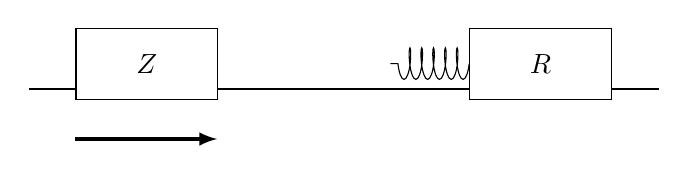
\begin{tikzpicture}
        %% Track
        \draw[thick] (-4,0) -- (4,0);
        %% Carts
        \node[draw,minimum width=1.8cm,minimum height=0.9cm,fill=white,anchor=base,yshift=2mm] (Z) at (-2.5,0) {$Z$};
        \node[draw,minimum width=1.8cm,minimum height=0.9cm,fill=white,anchor=base,yshift=2mm] (R) at (+2.5,0) {$R$};
        %% Spring
        \draw[decoration={aspect=0.2,segment length=1.5mm,amplitude=2mm,coil},decorate] (R.west) -- ++(180:1);
        %% Vector
        \draw[very thick,-latex] (Z.south west) ++(270:0.5) -- ++(0:1.8);
    \end{tikzpicture}
    \end{center}
    Car $R$ has a spring attached to it and is initially at rest.
    When the separation between the cars has reached a minimum, then:
    \begin{choices}
        \wrongchoice{car $R$ is still at rest.}
        \wrongchoice{car $Z$ has come to rest.}
        \wrongchoice{both cars have the same kinetic energy.}
        \wrongchoice{both cars have the same momentum.}
      \correctchoice{the kinetic energy of the system has reached a minimum.}
    \end{choices}
\end{question}
}

\element{aapt}{ %% Olympiad-A5
\begin{question}{olympiad-1998-q11}
    Two ice skaters, a \SI{200}{\pound} man and a \SI{120}{\pound} woman,
        are initially hugging on a frictionless level ice surface.
    Ten seconds after they push off from each other,
        they are \SI{8.0}{\meter} apart.
    How far has the woman moved in that time?
    \begin{multicols}{3}
    \begin{choices}
        \wrongchoice{\SI{8.0}{\meter}}
        \wrongchoice{\SI{6.5}{\meter}}
      \correctchoice{\SI{5.0}{\meter}}
        \wrongchoice{\SI{4.0}{\meter}}
        \wrongchoice{\SI{3.0}{\meter}}
    \end{choices}
    \end{multicols}
\end{question}
}

\element{aapt}{ %% Olympiad-A5
\begin{questionmult}{olympiad-1998-q12}
    %% to the right
    The diagram below shows the velocity-time graph for two masses $R$ and $S$ that collided elastically.
    \begin{center}
    \begin{tikzpicture}
        \begin{axis}[
            axis y line=left,
            axis x line=bottom,
            axis line style={->},
            xlabel={time},
            x unit=\si{\second},
            xtick={0,1,2,3,4},
            minor x tick num=1,
            ylabel={velocity},
            y unit=\si{\meter\per\second},
            ytick={0.0,0.4,0.8,1.2},
            minor y tick num=1,
            grid=major,
            xmin=0,xmax=4.05,
            ymin=0,ymax=1.205,
            width=0.8\columnwidth,
            height=0.5\columnwidth,
        ]
        \addplot[line width=1pt,no marks] plot coordinates { (0,0.8) (1,0.8) (3,0.2) (4,0.2) };
        \node[anchor=south] at (axis cs:0.5,0.8) {$R$};
        \addplot[line width=1pt,no marks] plot coordinates { (0,0) (1,0) (3,1.0) (4,1.0) };
        \node[anchor=north] at (axis cs:3.5,1.0) {$S$};
        \end{axis}
    \end{tikzpicture}
    \end{center}
    Which of the following statements is true?
    \begin{choices}
      \correctchoice{$R$ and $S$ moved in the same direction after the collision.}
      \correctchoice{The velocities of $R$ and $S$ were equal at the mid-time of the collision.}
        \wrongchoice{The mass of $S$ was greater than the mass of $R$.}
        %% A. I only B. II only C. I & II only D. II & III only E. I, II & III
    \end{choices}
\end{questionmult}
}

\element{aapt}{ %% Olympiad-A5
\begin{question}{olympiad-1998-q13}
    %% NOTE: reworded
    %% Questions 13 and 14 refer to the motion of two blocks along a frictionless level track.
    Two blocks are in motion along a frictionless level track.
    Block \#1 (mass $m_1$) is initially moving with speed $v_0$.
    It collides with and sticks to an initially stationary block (\#2) of mass $m_2 = 9 m_1$.
    %% start question
    What is the speed of the two blocks after the collision?
    \begin{multicols}{3}
    \begin{choices}
        \wrongchoice{$v_0$}
        \wrongchoice{$\dfrac{9}{10} v_0$}
        \wrongchoice{$\dfrac{8}{9} v_0$}
        \wrongchoice{$\dfrac{1}{9} v_0$}
      \correctchoice{$\dfrac{1}{10} v_0$}
    \end{choices}
    \end{multicols}
\end{question}
}

\element{aapt}{ %% Olympiad-A5
\begin{question}{olympiad-1998-q14}
    %%  NOTE: reword
    %% Questions 13 and 14 refer to the motion of two blocks along a frictionless level track.
    Two blocks are in motion along a frictionless level track.
    Block \#1 (mass $m_1$) is initially moving with speed $v_0$.
    It collides with and sticks to an initially stationary block (\#2) of mass $m_2 = 9 m_1$.
    %% start question
    What fraction of the initial kinetic energy of the system is converted to other forms (heat, sound, \ldots) as a result of the collision?
    \begin{multicols}{3}
    \begin{choices}
        \wrongchoice{\SI{1}{\percent}}
        \wrongchoice{\SI{10}{\percent}}
        \wrongchoice{\SI{50}{\percent}}
      \correctchoice{\SI{90}{\percent}}
        \wrongchoice{\SI{99}{\percent}}
    \end{choices}
    \end{multicols}
\end{question}
}


%% PhysicsOlympiad 1997
%%----------------------------------------
\element{aapt}{ %% Olympiad-A5
\begin{question}{olympiad-1997-q07}
    Three air track cars, shown in the accompanying figure,
        all have the same mass $m$.
    \begin{center}
    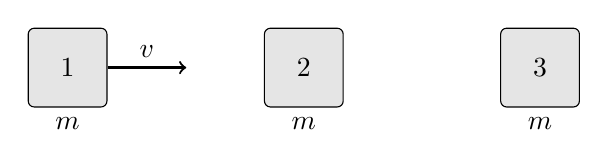
\begin{tikzpicture}
        %% Blocks
        \node[draw,minimum size=1cm,rounded corners=0.5ex,fill=white!90!black] (A) at (-3,0) {1};
        \node[draw,minimum size=1cm,rounded corners=0.5ex,fill=white!90!black] (B) at (+0,0) {2};
        \node[draw,minimum size=1cm,rounded corners=0.5ex,fill=white!90!black] (C) at (+3,0) {3};
        %% masses ??
        \node[anchor=north] at (A.south) {$m$};
        \node[anchor=north] at (B.south) {$m$};
        \node[anchor=north] at (C.south) {$m$};
        %% Arrows
        \draw[thick,->] (A.east) -- ++(0:1cm) node[pos=0.5,anchor=south] {$v$};
    \end{tikzpicture}
    \end{center}
    Cars 2 and 3 are initially at rest.
    Car 1 is moving to the right with speed $v$.
    Car 1 collides with car 2 and sticks to it.
    The 1-2 combination collides elastically with car 3.
    Which of the following is most nearly the final speed of car 3?
    \begin{multicols}{3}
    \begin{choices}
        \wrongchoice{$0.17 v$}
        \wrongchoice{$0.50 v$}
      \correctchoice{$0.67 v$}
        \wrongchoice{$0.80 v$}
        \wrongchoice{$1.00 v$}
    \end{choices}
    \end{multicols}
\end{question}
}


%% PhysicsOlympiad 1996
%%----------------------------------------
\element{aapt}{ %% Olympiad-A5
\begin{questionmult}{olympiad-1996-q10}
    A small sphere is moving at a constant speed in a vertical circle.
    %Below is a list of quantities that could be used to describe some aspect of the motion of the sphere.
    Which of these quantities will change as this sphere moves around the circle?
    \begin{choices}
        %% ANS is E
        \wrongchoice{kinetic energy}
      \correctchoice{potential energy}
      \correctchoice{momentum}
    \end{choices}
\end{questionmult}
}

\element{aapt}{ %% Olympiad-A5
\begin{question}{olympiad-1996-q12}
    Three air track cars are initially placed as shown in the accompanying figure.
    Car $A$ has mass $m$ and initial velocity $v$ to the right.
    Car $B$ with mass $m$ and car C with mass $4m$ are both initially at rest.
    \begin{center}
    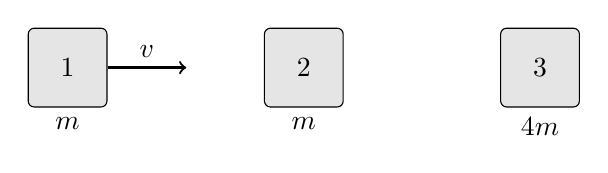
\begin{tikzpicture}
        %% Blocks
        \node[draw,minimum size=1cm,rounded corners=0.5ex,fill=white!90!black] (A) at (-3,0) {1};
        \node[draw,minimum size=1cm,rounded corners=0.5ex,fill=white!90!black] (B) at (+0,0) {2};
        \node[draw,minimum size=1cm,rounded corners=0.5ex,fill=white!90!black] (C) at (+3,0) {3};
        %% masses ??
        \node[anchor=north] at (A.south) {$m$};
        \node[anchor=north] at (B.south) {$m$};
        \node[anchor=north] at (C.south) {$4m$};
        %% Arrows
        \draw[thick,->] (A.east) -- ++(0:1cm) node[pos=0.5,anchor=south] {$v$};
    \end{tikzpicture}
    \end{center}
    Car $A$ collides elastically with car $B$,
        which in turn collides elastically with car $C$.
    After the collision, car $B$ is at rest.
    The final velocities of cars $A$ and $C$ are:
    \begin{choices}
      \correctchoice{Car $A$: $0.6v$ to the left; Car $C$: $0.4v$ to the right}
        \wrongchoice{Car $A$: $2.6v$ to the left; Car $C$: $0.4v$ to the right}
        \wrongchoice{Car $A$: at rest; Car $C$: $0.5v$ to the right}
        \wrongchoice{Car $A$: at rest; Car $C$: $0.25v$ to the right}
        \wrongchoice{Car $A$: at rest; Car $C$: $v$ to the right}
    \end{choices}
\end{question}
}


%% PhysicsOlympiad 1995
%%----------------------------------------
\element{aapt}{ %% Olympiad-A5
\begin{question}{olympiad-1995-q08}
    Car $A$ and car $B$ are both traveling down a straight highway at \SI{25}{\meter\per\second} (about \SI{56}{\mile\per\hour}).
    Car $A$ is only \SI{6.0}{\meter} behind car $B$.
    The driver of car $B$ brakes,
        slowing down with a constant acceleration of \SI{2.0}{\meter\per\second\squared}.
    After a time \SI{1.2}{\second},
        the driver of car $A$ begins to brake,
        also at \SI{2.0}{\meter\per\second\squared}.
    %% NOTE: make self contained
    %During the collision between car $A$ and car $B$ described in Problem \#7 above,
    During the collision between car $A$ and car $B$,
        which car experiences the greater change in momentum?
    \begin{choices}
        \wrongchoice{The more massive car.}
        \wrongchoice{The less massive car.}
        \wrongchoice{Car $A$ because its velocity at the start of the collision is greater.}
        \wrongchoice{Car $B$ because its velocity at the start of the collision is less.}
      \correctchoice{Both cars experience the same magnitude of momentum change.}
    \end{choices}
\end{question}
}

\element{aapt}{ %% Olympiad-A5
\begin{question}{olympiad-1995-q09}
    A \SI{70}{\kilo\gram} hunter ropes a \SI{350}{\kilo\gram} polar bear.
    Both are initially at rest,
        \SI{30}{\meter} apart on a frictionless and level ice surface.
    When the hunter pulls the polar bear to him,
        the polar bear will move:
    \begin{multicols}{3}
    \begin{choices}
      \correctchoice{\SI{5}{\meter}}
        \wrongchoice{\SI{6}{\meter}}
        \wrongchoice{\SI{15}{\meter}}
        \wrongchoice{\SI{24}{\meter}}
        \wrongchoice{\SI{25}{\meter}}
    \end{choices}
    \end{multicols}
\end{question}
}

\element{aapt}{ %% Olympiad-A5
\begin{question}{olympiad-1995-q10}
    A bullet of mass $m$ is fired at a block of mass $M$ initially at rest.
    The bullet, moving at an initial speed $v$,
        embeds itself in the block.
    The speed of the block after the collision is:
    \begin{multicols}{2}
    \begin{choices}
        \wrongchoice{$\dfrac{Mv}{M+m}$}
        \wrongchoice{$\dfrac{\left(M+m\right)v}{m}$}
        \wrongchoice{$v\sqrt{\dfrac{m}{M+m}}$}
        \wrongchoice{$v\sqrt{\dfrac{M+m}{m}}$}
      \correctchoice{$\dfrac{mv}{M+m}$}
    \end{choices}
    \end{multicols}
\end{question}
}


%% PhysicsOlympiad 1994
%%----------------------------------------
\element{aapt}{ %% Olympiad-A5
\begin{question}{olympiad-1994-q06}
    Three air track cars,
        shown in the accompanying figure,
        all have the same mass $m$.
    Cars 2 and 3 are initially at rest.
    Car 1 is moving to the right with speed $v$.
    \begin{center}
    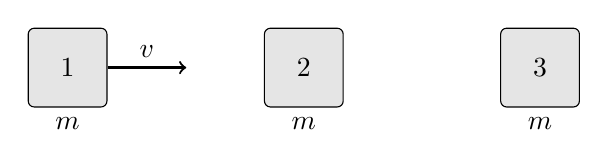
\begin{tikzpicture}
        %% Blocks
        \node[draw,minimum size=1cm,rounded corners=0.5ex,fill=white!90!black] (A) at (-3,0) {1};
        \node[draw,minimum size=1cm,rounded corners=0.5ex,fill=white!90!black] (B) at (+0,0) {2};
        \node[draw,minimum size=1cm,rounded corners=0.5ex,fill=white!90!black] (C) at (+3,0) {3};
        %% masses ??
        \node[anchor=north] at (A.south) {$m$};
        \node[anchor=north] at (B.south) {$m$};
        \node[anchor=north] at (C.south) {$m$};
        %% Arrows
        \draw[thick,->] (A.east) -- ++(0:1cm) node[pos=0.5,anchor=south] {$v$};
    \end{tikzpicture}
    \end{center}
    Car 1 collides with car 2 and sticks to it.
    The 1-2 combination collides elastically with car 3.
    Which of the following is most nearly the final speed of the 1-2 combination?
    \begin{multicols}{3}
    \begin{choices}
      \correctchoice{$0.17 v$}
        \wrongchoice{$0.50 v$}
        \wrongchoice{$0.67 v$}
        \wrongchoice{$0.80 v$}
        \wrongchoice{$1.0 v$}
    \end{choices}
    \end{multicols}
\end{question}
}

\endinput


